\documentclass[10pt,pdf,hyperref={unicode}]{beamer}

\mode<presentation>
{
\usetheme{boxes}
\beamertemplatenavigationsymbolsempty

\setbeamertemplate{footline}[page number]
\usecolortheme{seagull}
\setbeamersize{text margin left=0.5em, text margin right=0.5em}
}

\usepackage[utf8]{inputenc}
\usepackage[english, russian]{babel}
\usepackage{bm}
\usepackage{multirow}
\usepackage{ragged2e}
\usepackage{indentfirst}
\usepackage{multicol}

\usepackage{graphicx}
\usepackage{caption}
\usepackage{subcaption}


\newtheorem{rustheorem}{Теорема}

\AtBeginEnvironment{figure}{\setcounter{subfigure}{0}}% Resets subfigure counter at start of figure environment

%----------------------------------------------------------------------------------------------------------
\title[\hbox to 56mm{Обучение с экспетом\hfill\insertframenumber\,/\,\inserttotalframenumber}]
{Задача обучения с экспертом для построение\\ интерпретируемых моделей машинного обучения}
\author[А.\,В.~Грабовой]{\large Грабовой Андрей Валериевич}
\institute{\large
Московский физико-технический институт}

\date{\footnotesize{МФТИ, г. Москва}}
%----------------------------------------------------------------------------------------------------------

\begin{document}
%----------------------------------------------------------------------------------------------------------
\begin{frame}
\titlepage
\end{frame}

%----------------------------------------------------------------------------------------------------------
\begin{frame}{Вероятностная интерпретация дистилляции моделей}
\justifying
\textbf{Цель}

Предложить постановку задачи обучения с \textit{экспертной информацией} для обучения интерпретируемых моделей машинного обучения. 

~\\
\textbf{Задачи}

\begin{enumerate}
\justifying
	\item Поставить задачу обучения с экспертной информацией.
	\item Предложить метод решения предложенной задачи.
	\item Провести анализ предложенного метода для задачи аппроксимации кривых второго порядка.
\end{enumerate}

~\\
\textbf{Исследуемая проблема}

Построение интерпретируемых моделей глубокого обучения.

\end{frame}

%----------------------------------------------------------------------------------------------------------
\begin{frame}{Список литературы}
\justifying
\begin{enumerate}
	\item \textit{Грабовой А.В., Стрижов В.В.} Анализ свойств вероятностных моделей обучения с экспертом~// в процессе подачи.
	\item \textit{Грабовой А.В., Стрижов В.В.} Анализ выбора априорного распределения для смеси экспертов // Журнал Вычислительной математики и математической физики, 2021. Т.\,61. \textnumero\,5.
	\item \textit{Yuksel Seniha Esen, Wilson Joseph N., Gader Paul D} Twenty Years of Mixture of Experts~// IEEE Transactions on Neural Networks and Learning Systems, 2012. Vol.\,23. No\,8. Pp.\,1177--1193.
\end{enumerate}
\end{frame}

%----------------------------------------------------------------------------------------------------------

\begin{frame}{Обучение с экспертной информацией}
\justifying
\begin{center}
	\includegraphics[width=0.9\textwidth]{figures/explanation}
\end{center}

\begin{enumerate}
    \item Учитель~$\mathbf{f}$ влияет на выбор ученика~$\mathbf{g}$ в пространстве~$x$.
    \item Учитель~$\mathbf{f}_1$ корректирует шумные данные в $x$.
    \item Модель учителя~$\mathbf{f}_2$ более сложная, поэтому она аппроксимирует также и шум.
\end{enumerate}

\end{frame}

%----------------------------------------------------------------------------------------------------------

\begin{frame}{Постановка задачи: кривые второго порядка}
\justifying
Изображение
\[
\mathbf{M} \in \{0,1\}^{m_1\times m_2},
\]
где $1$~--- точка изображение,  а $0$~--- точка фона. 

Точки изображения --- кривая второго порядка~$\Omega$.

Координаты точек изображения $\mathbf{C} \in \mathbb{R}^{N\times2}$.

Экспертная информация о фигуре~$\Omega$ обозначается $E\bigr(\Omega\bigr)$.

Построение новой задачи:
\[
K_x\bigr(E\bigr(\Omega\bigr)\bigr):\mathbb{R}^{2} \to \mathbb{R}^{n},
\quad K_y\bigr(E\bigr(\Omega\bigr)\bigr): \mathbb{R}^{2} \to \mathbb{R},
\]
где $K_x, K_y$ отображения объектов в признаковое описание и пространство ответов.

Выборка для аппроксимации:
\[
\mathfrak{D} = \{(\mathbf{x}, y) \; | \; \forall \mathbf{c} \in \mathbf{C} \; \mathbf{x} = K_x(\mathbf{c}), \; y = K_y(\mathbf{c}) \}.
\]

В данной работе предполагается, что выборка~$\mathfrak{D}$ аппроксимируется линейной моделью:
\[
	g(\mathbf{x}, \mathbf{w}) = \mathbf{x}^\mathsf{T} \mathbf{w},
\]
где~$\mathbf{w}$ вектор, параметр, который требуется найти.


Требуется решить следующую оптимизационную задачу:
\[
	\hat{\mathbf{w}} = \arg\min_{\mathbf{w}\in\mathbb{R}^n} \sum_{\left(\mathbf{x}, y\right) \in \mathfrak{D}}\|g(\mathbf{x}, \mathbf{w}) - y \|_2^2.
\]
\end{frame}

%----------------------------------------------------------------------------------------------------------

\begin{frame}{Постановка задачи: признаковое описание кривых}
\justifying
Произвольная кривая второго порядка, главная ось которой не параллельна оси ординат, задается следующим выражением:
\[
\label{st:coef}
x^2 = B'xy+C'y^2+D'x+E'y+F',
\]
где на коэффициенты $B',C'$ накладываются ограничения, которые зависят от вида кривой. 

Также получаем:
\[
K_x\bigr(\mathbf{c}_i\bigr)=\left[x_iy_i, y_i^2, x_i, y_i, 1\right], \quad K_y\bigr(\mathbf{c}_i\bigr)=x_i^2,
\]
откуда получаем задачу линейной регрессии для восстановления параметров:
\[
B', C', D', E', F'
\] по выборке $\mathfrak{D}$.
\end{frame}

%----------------------------------------------------------------------------------------------------------

\begin{frame}[shrink=5]{Постановка задачи нахождения параметров окружностей}
\justifying
\begin{columns}
\column{0.6\textwidth}
Задано бинарное изображение:
\begin{equation*}
\begin{aligned}
\textbf{M} \in \{0,1\}^{m_1 \times m_2},
\end{aligned}
\end{equation*}
где $1$ --- черная точка, $0$ --- белая точка фона.

По изображению $\textbf{M}$ строится выборка $\textbf{C}$:
\begin{equation*}
\begin{aligned}
\textbf{C} \in  \mathbb{R}^{N \times 2},
\end{aligned}
\end{equation*}
где $N$ --- число черных точек на изображении $\textbf{M}$.
\column{0.36\textwidth}
\begin{center}
	\includegraphics[height=0.4\textheight]{figures/slides_statment}
\end{center}
\end{columns}


Пусть $x_0, y_0$~--- центр окружности, которую требуется найти, а $r$ ее радиус.

Точки~$\left(x_i, y_i\right)\in\textbf{C}$ должны удовлетворять уравнению окружности:
\begin{equation*}
\begin{aligned}
\left(x_i - x_0\right)^{2}+\left(y_i-y_0\right)^2 = r^2 \Rightarrow (2x_0)\cdot x_i + (2y_0)\cdot y_i+(r^2-x_0^2-y_0^2)\cdot1 = x_{i}^2 + y_{i}^2.
\end{aligned}
\end{equation*}
Задачу линейной регрессии для нахождения окружности:
\begin{equation*}
\begin{aligned}
\textbf{X}\textbf{w} \approx \textbf{y},  \quad \textbf{X} = \left[\textbf{C}, \textbf{1}\right], \quad \textbf{y} = [x_1^2+y_1^2, x_2^2+y_2^2, \cdots, x_N^2+y_N^2]^{\mathsf{T}},
\end{aligned}
\end{equation*}
где найденые оптимальные параметры линейной регрессии $\textbf{w} = \bigr[w_1, w_2, w_3\bigr]^{\mathsf{T}}$ восстанавливают параметры окружности:
\begin{equation*}
\begin{aligned}
x_0 = \frac{w_1}{2}, \quad y_0 = \frac{w_2}{2}, \quad r = \sqrt[]{w_3+x_{0}^{2}+y_{0}^{2}}.
\end{aligned}
\end{equation*}

\end{frame}

%----------------------------------------------------------------------------------------------------------

\begin{frame}{Постановка задачи: мультимодель}
\justifying
Заданы $K$ кривых второго порядка $\Omega_1, \cdots, \Omega_K$ с $E_k = E\bigr(\Omega_k\bigr)$.

\begin{definition}
Функция $f$ называется смесью K экспертов, если:
\[
	f = \sum\limits_{k = 1}^{K}\pi_k(\mathbf{x}, \mathbf{V})g_k(\mathbf{w}_k),  \quad \pi_k(\mathbf{x}, \mathbf{V}): \mathbb{R}^{n\times |\mathbf{V}|} \rightarrow [0, \, 1], \quad \sum\limits_{k = 1}^{K}\pi_k(\mathbf{x}, \mathbf{V}) = 1, 
\]
где $g_k$~---~локальная модель, $\mathbf{x}$~---~признаки, $\pi_k$~---~шлюзовая функция, $\mathbf{w}_k$~---~параметры, $\mathbf{V}$~---~параметры шлюзовой функции.
\end{definition}

Мультимодель, описывающую кривые $\Omega_1, \dots, \Omega_K$ на изображении $\mathbf{M}$:
\[
\setlength\abovedisplayskip{0pt}
	f = \sum\limits_{\mathbf{c} \in \mathbf{C}} \sum_{k = 1}^{K} \pi_k(\mathbf{c}, \mathbf{V})g_k(K^k_{x}\bigl(\mathbf{c}), \mathbf{w}_k), \quad \mathbf{x}=K^1_{x}\bigl(\mathbf{c})=\cdots=K^K_{x}\bigl(\mathbf{c}).
\setlength\belowdisplayskip{0pt}
\]
Решается задача оптимизации:
\[
\setlength\abovedisplayskip{0pt}
\mathcal{L} = \sum\limits_{(\mathbf{x}, y) \in \mathfrak{D}} \sum\limits_{k = 1}^{K} \pi_k(\mathbf{x}, \mathbf{V})(y - \mathbf{w}_k^{\mathsf{T}}\mathbf{x})^2 + R\bigl(\mathbf{V}, \mathbf{W}, E(\Omega)\bigr) \rightarrow \min_{\mathbf{V}, \mathbf{W}},
\setlength\belowdisplayskip{0pt}
\]
где $\mathbf{W} = [\mathbf{w}_1, \dots, \mathbf{w}_k]$~--- параметры локальных моделей, $R\bigl(\mathbf{V}, \mathbf{W}, E(\Omega)\bigr)$~---~регуляризация параметров, основанная на экспертной информации.

\end{frame}

%----------------------------------------------------------------------------------------------------------

\begin{frame}{Вероятностная задача}
\justifying

Рассматривается вероятностная постановка задачи:
\begin{enumerate}
	\item[1)] правдоподобие выборки $p_{k}\left(y_{i}|\mathbf{w}_{k}, \mathbf{x}_{i}\right) = \mathcal{N}\left(y_{i}|\mathbf{w}_{k}^{\mathsf{T}}\mathbf{x}_{i}, \beta^{-1}\right),$ где $\beta$ уровень шума,
	\item[2)] априорное распределение параметров $p^{k}\left(\mathbf{w}_{k}\right) = \mathcal{N}\left(\mathbf{w}_{k}|\mathbf{w}^{0}_{k}, \mathbf{A}_{k}\right),$ где $\mathbf{w}^{0}_{k}$~---~вектор размера $n\times1,$ $\mathbf{A}_{k}$~---~ковариационная матрица параметров,
	\item[3)] регуляризация априорного распределения $p\left(\bm{\varepsilon}_{k,k'}|\bm{\alpha}\right) = \mathcal{N}\left(\bm{\varepsilon}_{k,k'}|\mathbf{0},  \bm{\Xi}\right),$ где~$\bm{\Xi}$~---~ковариационная матрица общего вида, $\bm{\varepsilon}_{k,k'} = \mathbf{w}_{k}^{0}-\mathbf{w}_{k'}^{0}.$
\end{enumerate}

Правдоподобие модели включает правдоподобие выборки, априорное распределение параметров, а также их регуляризацию
\[
\begin{aligned}
p\bigr(\mathbf{y}, \mathbf{W}|\mathbf{X}, \mathbf{V}, \textbf{A}, \textbf{W}^{0}, \bm{\Xi}, \beta\bigr) = &\prod_{k,k'=1}^{K}\mathcal{N}\left(\bm{\varepsilon}_{k,k'}|\mathbf{0},  \bm{\Xi}\right)\cdot\\
&\cdot\prod_{k=1}^{K}\mathcal{N}\left(\mathbf{w}_{k}|\mathbf{w}^{0}_{k}, \mathbf{A}_{k}\right)\prod_{i=1}^{N}\left(\sum_{k=1}^{K}\pi_{k}\mathcal{N}\left(y_{i}|\mathbf{w}_{k}^{\mathsf{T}}\mathbf{x}_{i}, \beta^{-1}\right)\right),
\end{aligned}
\]
где~$\mathbf{A} = \bigr\{\mathbf{A}_1, \cdots, \mathbf{A}_K\bigr\}.$

\end{frame}

%----------------------------------------------------------------------------------------------------------

\begin{frame}{ЕМ--алгоритм решения задачи}
\justifying

Введем скрытые переменные $\textbf{Z} = [z_{ik}],$ где $~z_{ik} = 1$ тогда и только тогда, когда $k_i=k$:
\[
\begin{aligned}
\log p\bigr(\mathbf{y}, \mathbf{Z}, \mathbf{W}&|\mathbf{X}, \mathbf{V}, \textbf{A}, \textbf{W}^{0},  \bm{\Xi}, \beta\bigr) =\\
&= \sum_{i=1}^{N}\sum_{k=1}^{K}z_{ik}\left[\log\pi_k\left(\textbf{x}_i, \textbf{V}\right) - \frac{\beta}{2}\left(y_{i} - \textbf{w}_{k}^{\mathsf{T}}\textbf{x}_{i}\right)^{2} + \frac{1}{2}\log\frac{\beta}{2\pi}\right] +\\
&+ \sum_{k=1}^{K}\left[-\frac{1}{2}\left(\textbf{w}_{k} - \textbf{w}_{k}^{0}\right)^{\mathsf{T}}\textbf{A}_{k}^{-1}\left(\textbf{w}_{k} - \textbf{w}_{k}^{0}\right) + \frac{1}{2}\log\det\textbf{A}^{-1}_{k} - \frac{n}{2}\log2\pi\right]+\\
&+ \sum_{k=1}^{K}\sum_{k'=1}^{K}\left[-\frac{1}{2}\left(\textbf{w}_{k}^{0}-\textbf{w}_{k'}^{0}\right)^{\mathsf{T}}\hat{\bm{\alpha}}^{-1}\left(\textbf{w}_{k}^{0}-\textbf{w}_{k'}^{0}\right) +\frac{1}{2}\log\det \bm{\Xi} -\frac{n}{2}\log{2\pi}\right].
\end{aligned}
\]

Задача оптимизации параметров локальных моделей и параметров смеси принимает следующий вид:
\begin{equation*}
\begin{aligned}
\mathbf{W}, \mathbf{Z}, \mathbf{V}, \mathbf{W}^0, \textbf{A},  \beta = \arg\max_{\mathbf{W}, \mathbf{Z}, \mathbf{V}, \mathbf{W}^0, \textbf{A}, \beta} \log p\bigr(\mathbf{y}, \mathbf{Z}, \mathbf{W}&|\mathbf{X}, \mathbf{V}, \textbf{A}, \textbf{W}^{0}, \bm{\Xi}, \beta\bigr).
\end{aligned}
\end{equation*}

Для оптимизации используется вариационный ЕМ--алгоритм с предположением~$q\left(\textbf{Z}, \textbf{W}\right) = q\left(\textbf{Z}\right)q\left(\textbf{W}\right)$.
\end{frame}

%----------------------------------------------------------------------------------------------------------
\begin{frame}{EM--алгоритм для решения задачи смеси экспертов}
\justifying
Итерационные формулы ЕМ--алгоритма:
	\begin{enumerate}
		\item Е--шаг: 
			\begin{equation*}
				\begin{aligned}
					&p\left(z_{ik} = 1\right) = \frac{\exp\left(\log\pi_{k}\left(\textbf{x}_{i}, \textbf{V}\right) - \frac{\beta}{2}\left(\textbf{x}_{i}^{\mathsf{T}}\mathsf{E}\textbf{w}_{k}\textbf{w}_{k}^{\mathsf{T}}\textbf{x}_{i} - \textbf{x}_{i}^{\mathsf{T}}\mathsf{E}\textbf{w}_{k}\right)\right)}{\sum_{k'=1}^{K}\exp\left(\log\pi_{k'}\left(\textbf{x}_{i}, \textbf{V}\right) - \frac{\beta}{2}\left(\textbf{x}_{i}^{\mathsf{T}}\mathsf{E}\textbf{w}_{k'}\textbf{w}_{k'}^{\mathsf{T}}\textbf{x}_{i} - \textbf{x}_{i}^{\mathsf{T}}\mathsf{E}\textbf{w}_{k'}\right) \right)},\\
					&q(\textbf{w}_k) = \mathcal{N}(\textbf{w}_k|\textbf{m}_k, \textbf{B}_k),\\
					&\mathbf{m}_{k} = \mathbf{B}_{k}\left(\mathbf{A}_{k}^{-1}\mathbf{w}_{k}^{0}+\beta\sum_{i=1}^{N}\mathbf{x}_{i}y_{i}\mathsf{E}z_{ik}\right), \quad
					\mathbf{B}_{k} = \left(\mathbf{A}_{k}^{-1}+\beta\sum_{i=1}^{N}\mathbf{x}_{i}\mathbf{x}_{i}^{\mathsf{T}}\mathsf{E}z_{ik}\right)^{-1} .
				\end{aligned}
			\end{equation*}
		\item М--шаг: 
			\begin{equation*}
				\begin{aligned}
					&\textbf{A}_{k} = \mathsf{E}\textbf{w}_{k}\textbf{w}_{k}^{\mathsf{T}} - \textbf{w}_{k}^{0}\mathsf{E}\textbf{w}_{k}^{\mathsf{T}} - \mathsf{E}\textbf{w}_{k}\textbf{w}_{k}^{0\mathsf{T}} + \textbf{w}_{k}^{0}\textbf{w}_{k}^{0\mathsf{T}}, \\
					 &\frac{1}{\beta}=\frac{1}{N}\sum_{i=1}^{N}\sum_{k=1}^{K}\left[y_{i}^{2}-2y_{i}\textbf{x}_{i}^{\mathsf{T}}\mathsf{E}\textbf{w}_{k} + \textbf{x}_{i}^{\mathsf{T}}\mathsf{E}\textbf{w}_{k}\textbf{w}_{k}^{\mathsf{T}}\textbf{x}_{i}\right]\mathsf{E}z_{ik},\\
					&\textbf{w}_{k}^{0} =\left[\textbf{A}_{k}^{-1}+\left(K-1\right)\bm{\Xi}\right]^{-1}\left(\textbf{A}^{-1}_{k}\mathsf{E}\textbf{w}_{k}+\bm{\Xi}\sum_{k'=1,~k'\not=k}^{K}\textbf{w}_{k'}^{0}\right),\\
					&\textbf{V}= \arg\max_{\textbf{V}} \mathsf{E}_{q^{s}}\log p\bigr(\mathbf{y}, \textbf{Z},\mathbf{W}|\mathbf{X}, \mathbf{V}, \textbf{A}, \textbf{W}^{0}, \bm{\Xi}, \beta\bigr).
				\end{aligned}
			\end{equation*}
	\end{enumerate}
\end{frame}
%----------------------------------------------------------------------------------------------------------


\begin{frame}{Вычислительный эксперимент}
\justifying
\textbf{Эксперимент с окружностями:}

Информация

~\\
\textbf{Эксперимент с разным уровнем шума в данных:}

Информация

~\\
\textbf{Аппроксимация радужки глаза}

Информация

\end{frame}
%----------------------------------------------------------------------------------------------------------

\begin{frame}{Эксперимент с окружностями}
\justifying

\begin{figure}[h!]
\begin{minipage}{.32\textwidth}
      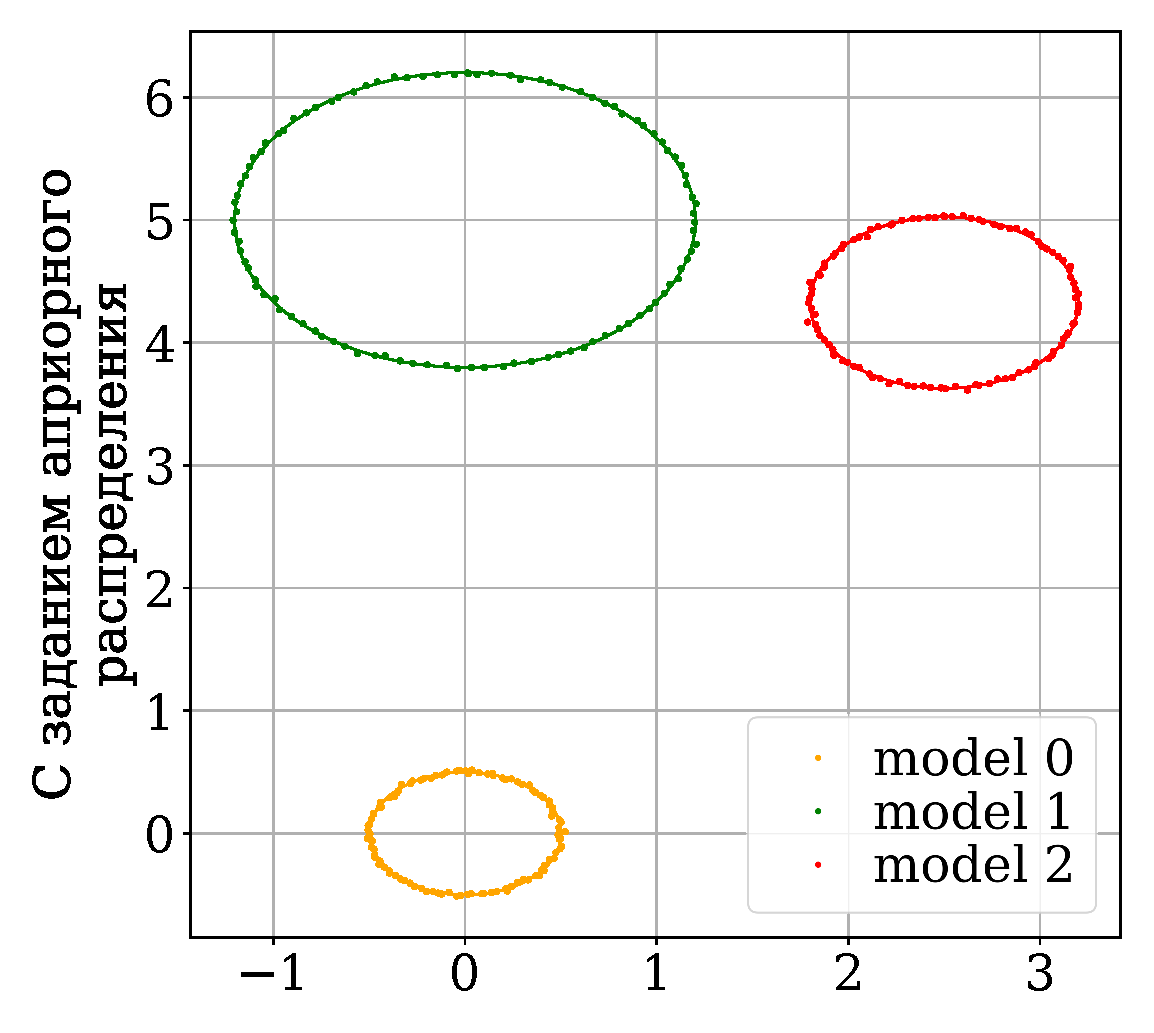
\includegraphics[width =  \textwidth]{figures/910.eps}
\end{minipage}
\begin{minipage}{.32\textwidth}
\hspace{0.3mm}
      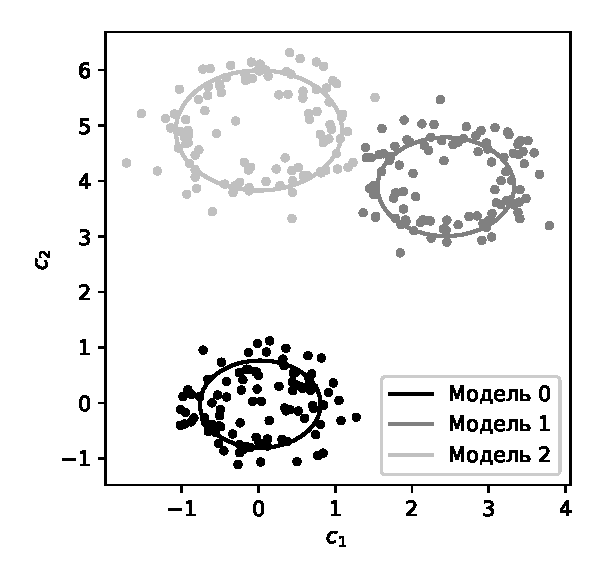
\includegraphics[width =  0.89\textwidth]{figures/901.eps}
\end{minipage}
\begin{minipage}{.32\textwidth}
\vspace{-3mm}
\hspace{-8.5mm}
      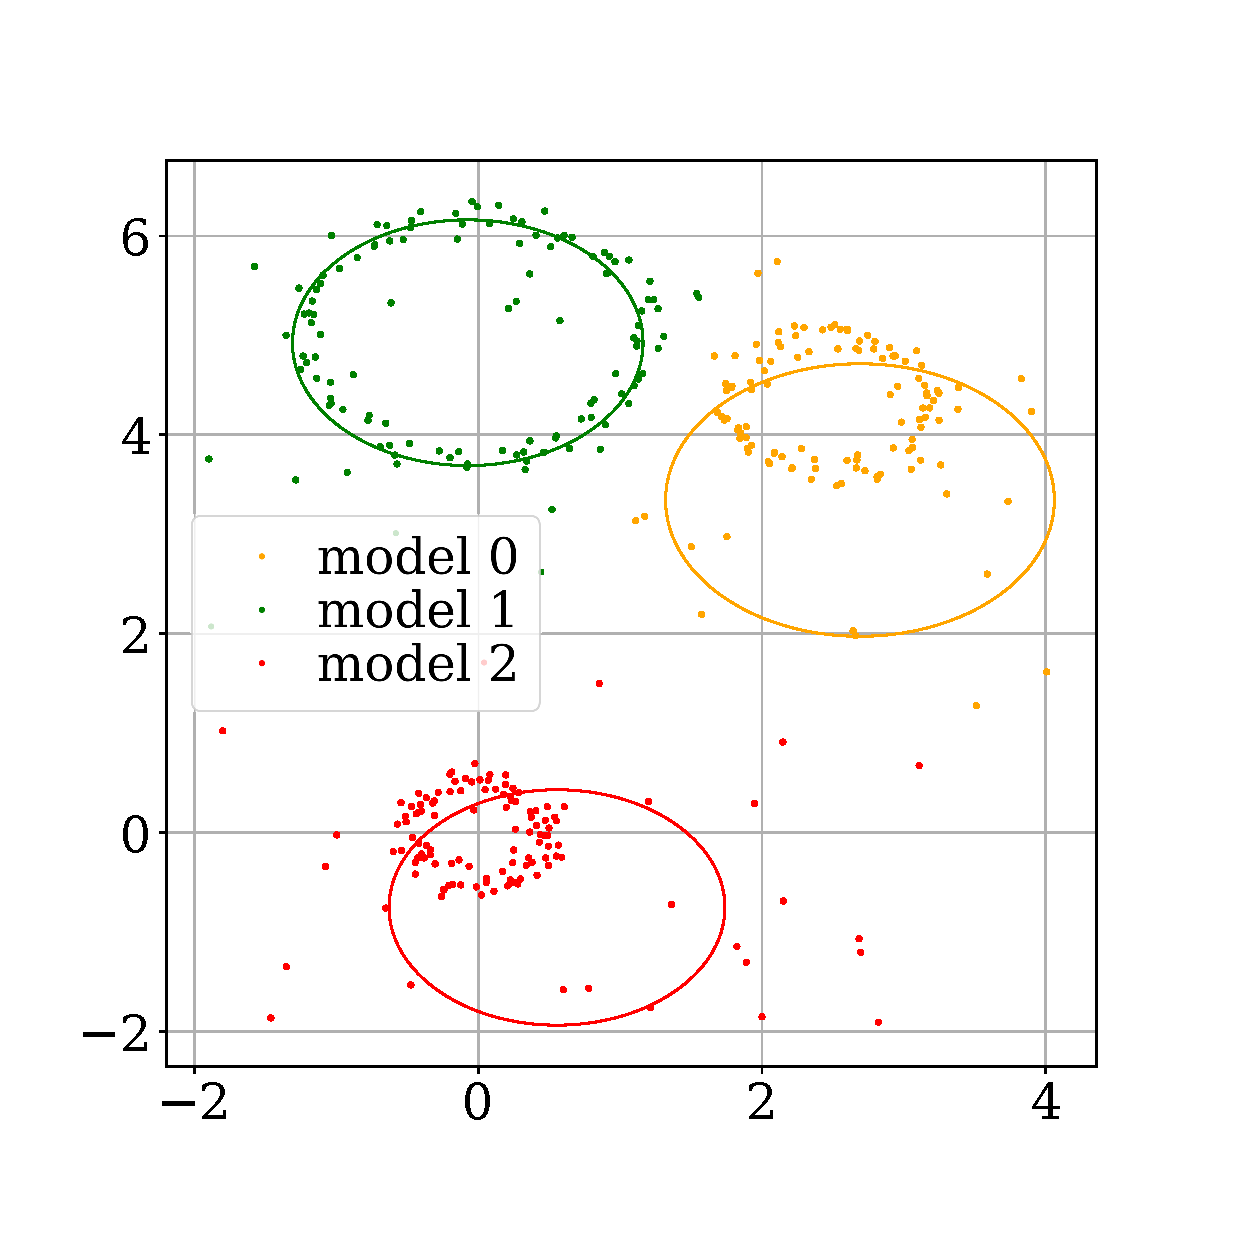
\includegraphics[width =  1.07\textwidth]{figures/902.eps}
\end{minipage}
\begin{minipage}{.32\textwidth}
      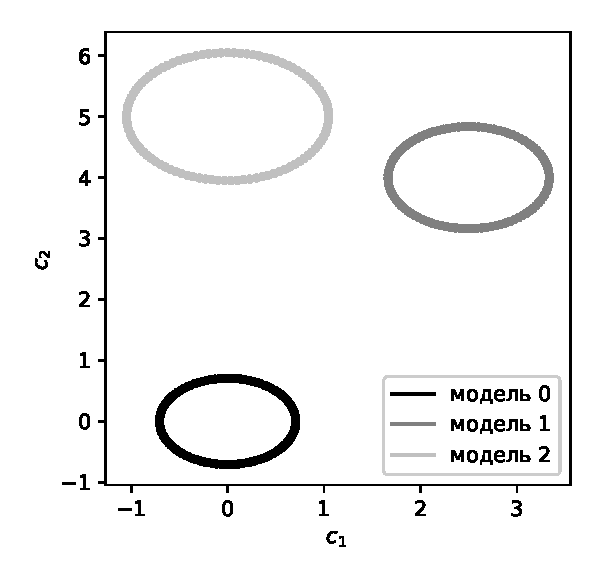
\includegraphics[width =  \textwidth]{figures/900.eps}
\end{minipage}
\begin{minipage}{.32\textwidth}
\hspace{2mm}
      \includegraphics[width =  0.9\textwidth]{figures/911.eps}
\end{minipage}
\begin{minipage}{.32\textwidth}
\hspace{-2.3mm}
      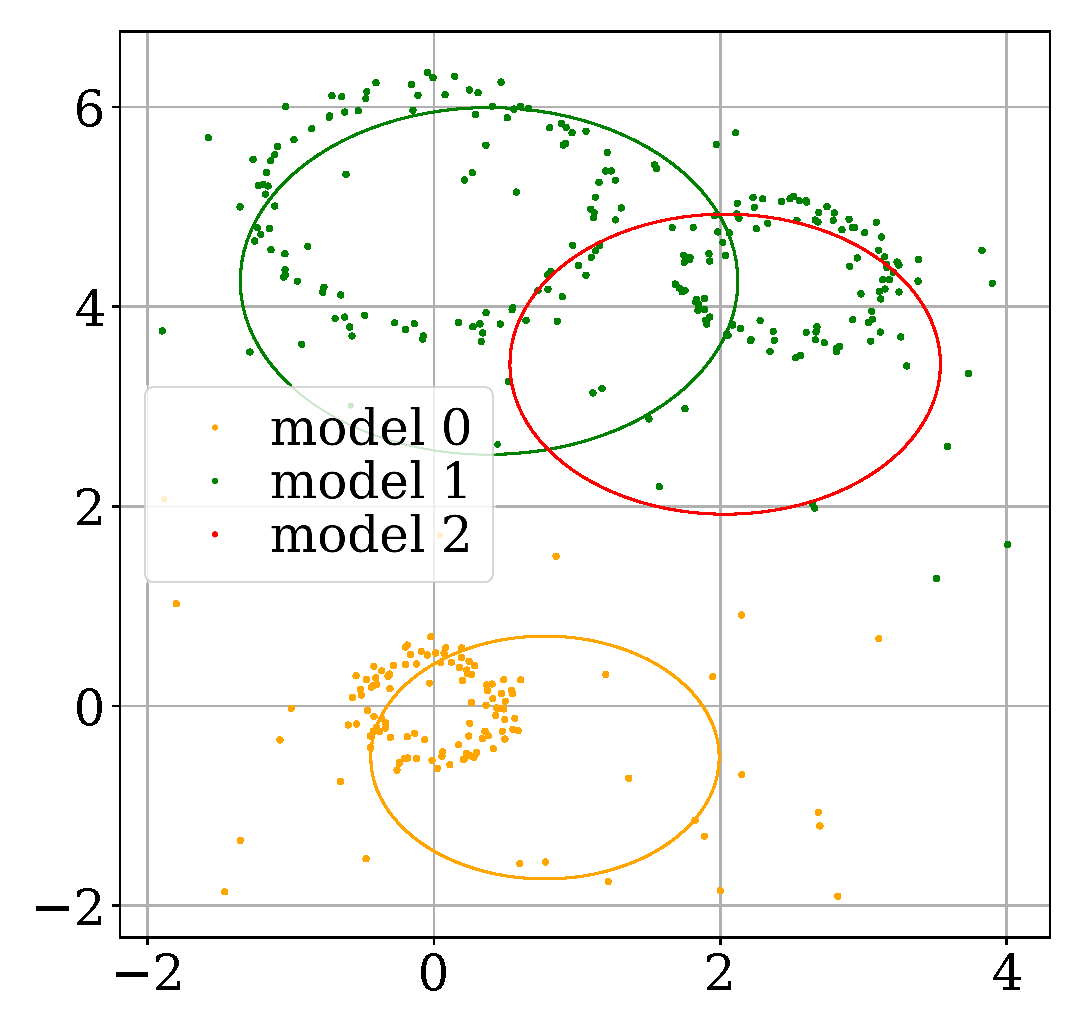
\includegraphics[width =  0.935\textwidth]{figures/912.eps}
\end{minipage}
\caption{Мультимодель в зависимости от разных априорных предположений и уровня шума. Сверху вниз: построение с заданием априорного распределения; без задания априорного распределения. Слева на право: окружности без шума; шум в радиусе окружности; шум в радиусе окружности а также произвольные точки по всему изображению.}
\label{ce:fig3}
\end{figure}


\end{frame}
%----------------------------------------------------------------------------------------------------------

\begin{frame}{Эксперимент с разным уровнем шума}
\justifying

\begin{figure}[h]
\begin{minipage}{.32\textwidth}
\hspace{-3mm}
      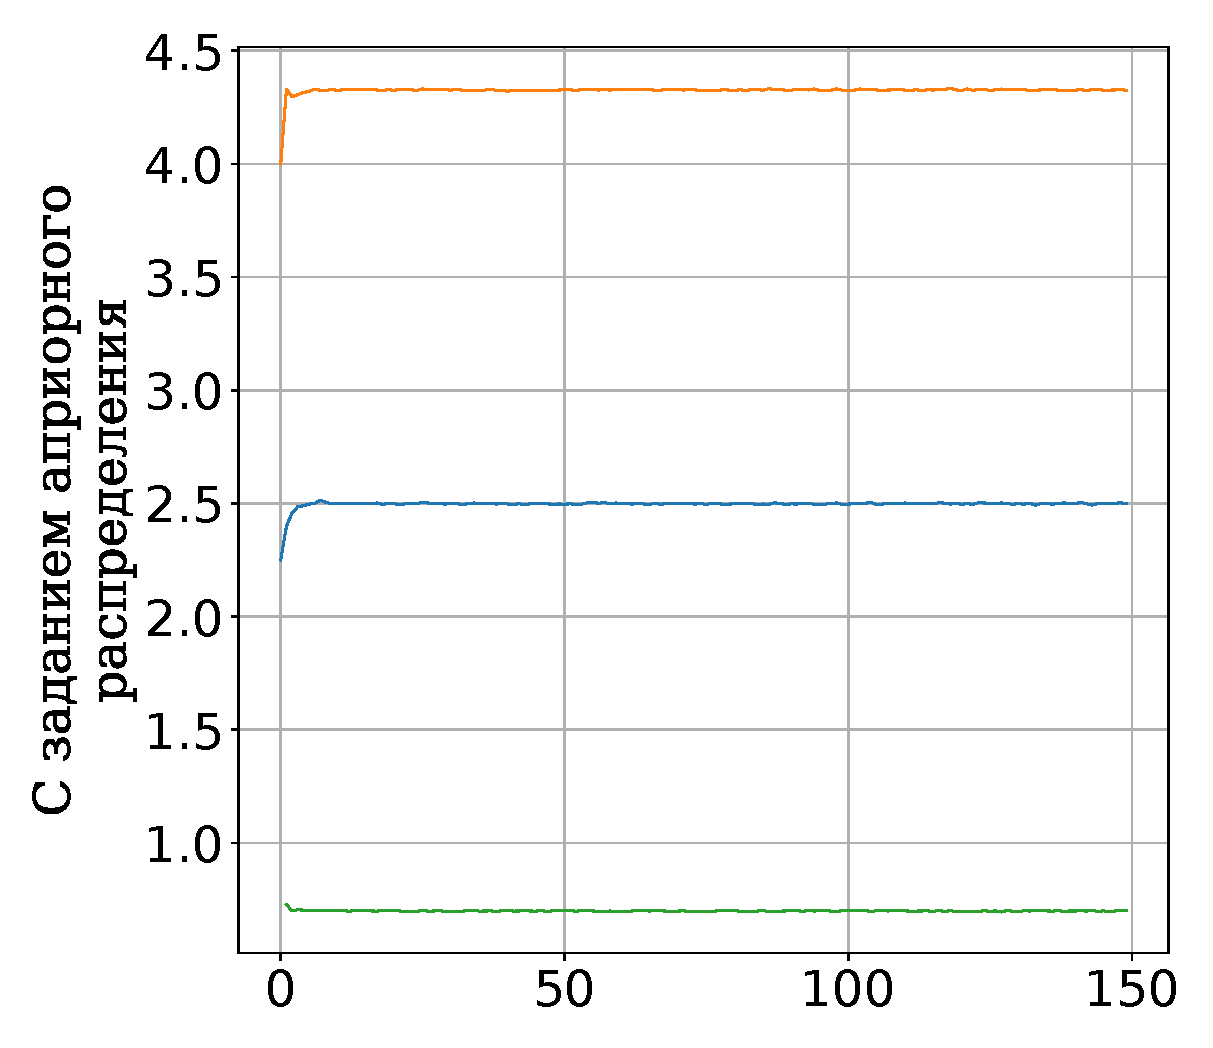
\includegraphics[width = 1.05\textwidth]{figures/910noise.eps}
\end{minipage}
\begin{minipage}{.32\textwidth}
\vspace{2pt}
\hspace{-2.1mm}
      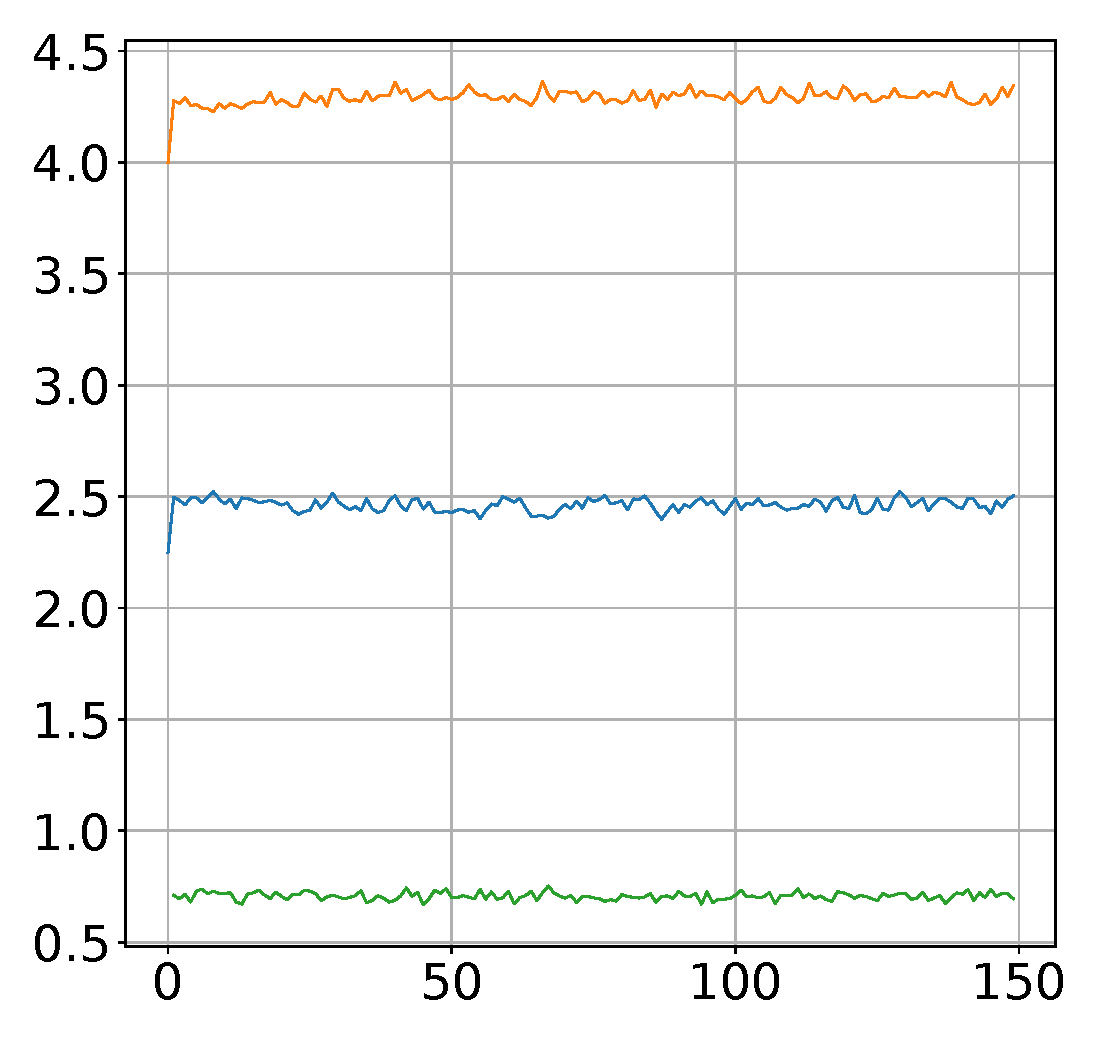
\includegraphics[width = 0.95\textwidth]{figures/911noise.eps}
\end{minipage}
\begin{minipage}{.32\textwidth}
\vspace{2pt}
\hspace{-6.3mm}
      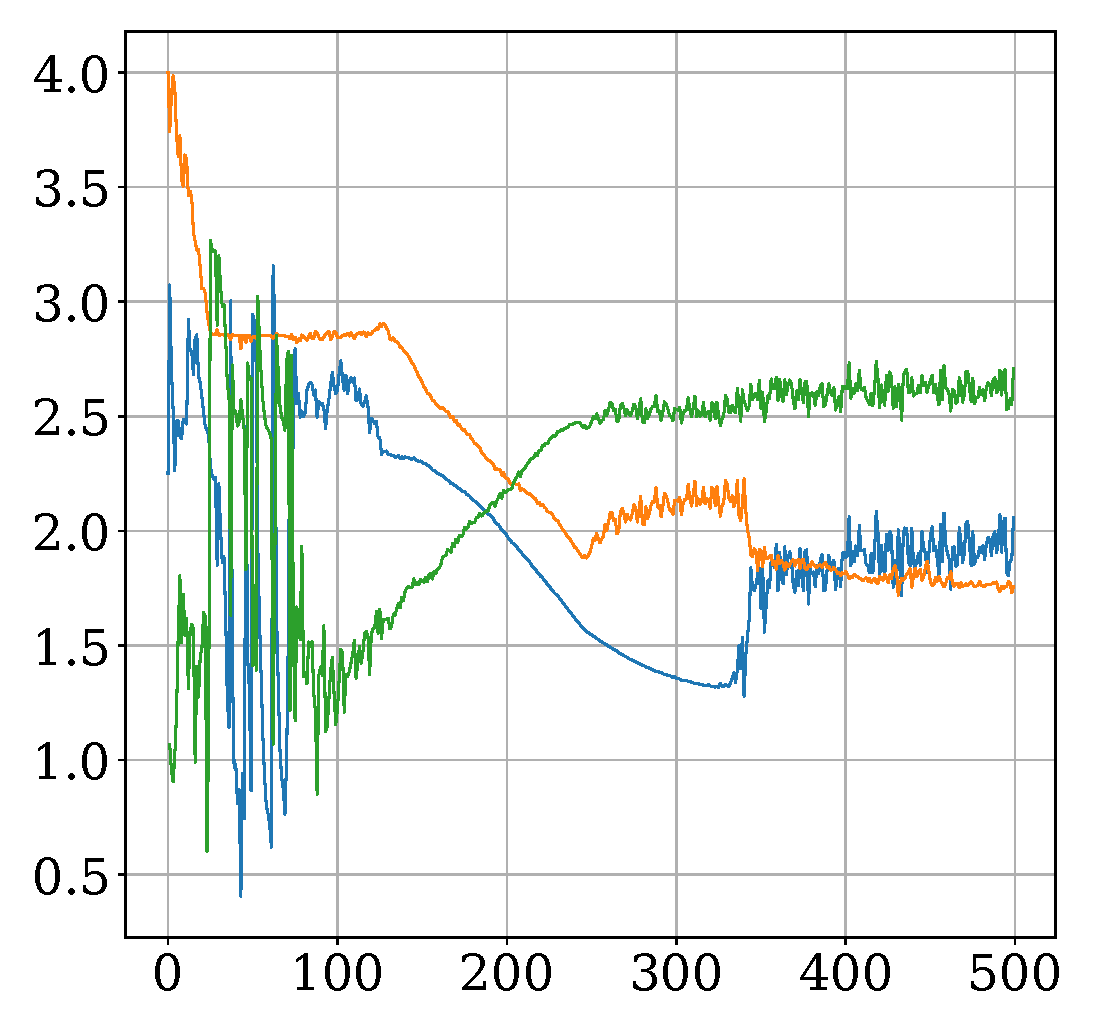
\includegraphics[width = 0.95\textwidth]{figures/912noise.eps}
\end{minipage}
\begin{minipage}{.32\textwidth}
\hspace{-3mm}
      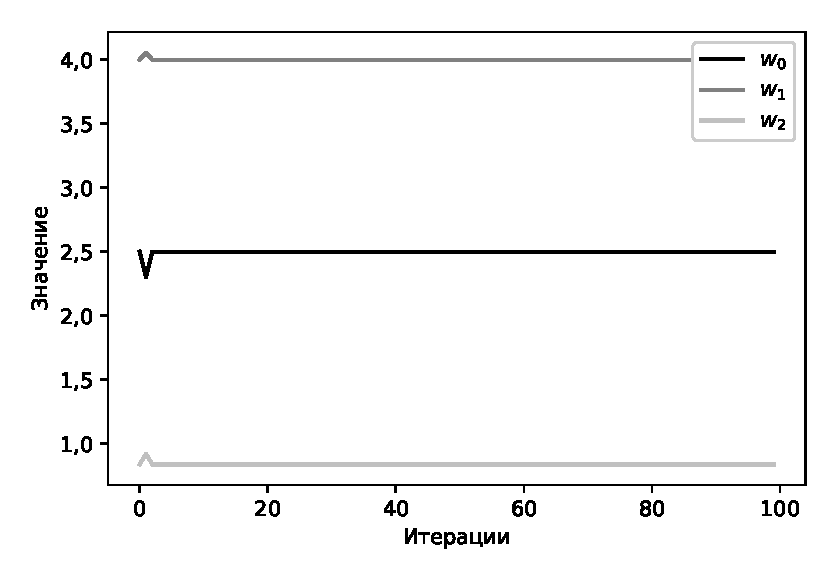
\includegraphics[width = 1.05\textwidth]{figures/900noise.eps}
\end{minipage}
\begin{minipage}{.32\textwidth}
\hspace{-2.1mm}
      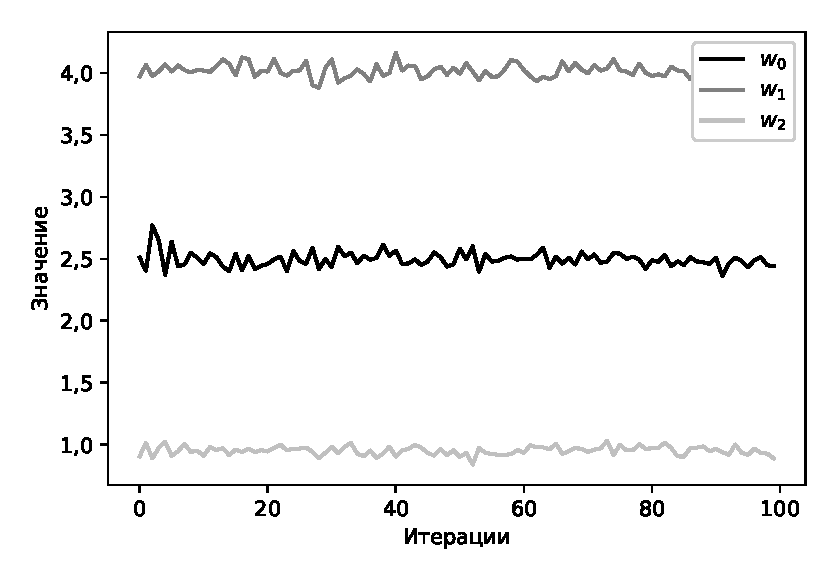
\includegraphics[width = \textwidth]{figures/901noise.eps}
\end{minipage}
\begin{minipage}{.32\textwidth}
\hspace{-2mm}
      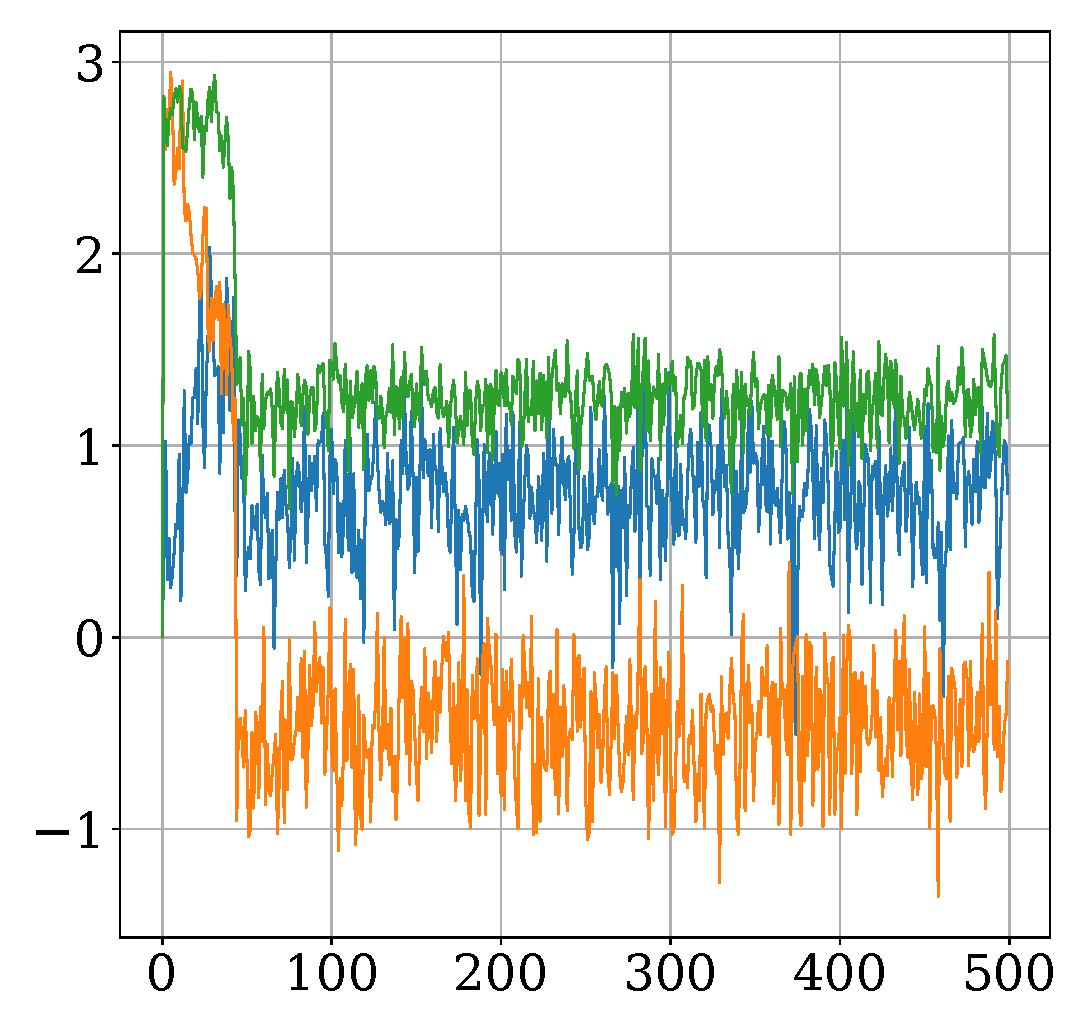
\includegraphics[width = 0.95\textwidth]{figures/902noise.eps}
\end{minipage}
\caption{Зависимость параметров $r$, $x_0$ и $y_0$ от номера итерации при разных априорных распределениях. Сверху вниз: построение с заданием априорного распределения; без задания априорного распределения. Слева на право: окружности без шума; шум в радиусе окружности; шум в радиусе окружности а также произвольные точки по всему изображению.}
\label{ce:fig4}
\end{figure}

\end{frame}
%----------------------------------------------------------------------------------------------------------

\begin{frame}{Эксперимент с разным уровнем шума}
\justifying

\begin{figure}[h!t]\center
\includegraphics[width=0.6\textwidth]{figures/beta_gamma}
\caption{Результат аппроксимации для данных с разным уровнем шума~$\beta$ и от дисперсии априорного распределения~$\gamma$}
\label{ce:fig6}
\end{figure}

\end{frame}
%----------------------------------------------------------------------------------------------------------

\begin{frame}{Эксперимент с разным уровнем шума}
\justifying

\begin{figure}[h!t]\center
\includegraphics[width=0.8\textwidth]{figures/3dplot}
\caption{Результат аппроксимации для данных с разным уровнем шума~$\beta$ и от дисперсии априорного распределения~$\gamma$}
\label{ce:fig6}
\end{figure}

\end{frame}
%----------------------------------------------------------------------------------------------------------

\begin{frame}{Эксперимент с аппроксимаций радужки глаза}
\justifying

\begin{figure}
     \centering
     \begin{subfigure}[b]{0.3\textwidth}
         \centering
         \includegraphics[width=\textwidth]{figures/not_prior_real_example}
         \caption{}
     \end{subfigure}
     \begin{subfigure}[b]{0.3\textwidth}
         \centering
         \includegraphics[width=\textwidth]{figures/prior_real_example}
         \caption{}
     \end{subfigure}
     \begin{subfigure}[b]{0.3\textwidth}
         \centering
         \includegraphics[width=\textwidth]{figures/prior_regular_real_example}
         \caption{}
     \end{subfigure}
     \caption{Визуализация аппроксимации радужки глаза: a) в случае, если задан регуляризатор $R_0$; b) в случае, если задан регуляризатор $R_1$; b) в случае, если задан регуляризатор $R_2$.}
    \label{ce:fig6}
\end{figure}

\end{frame}
%----------------------------------------------------------------------------------------------------------

\begin{frame}{Заключение}
\justifying
	\begin{enumerate}
	\justifying
		\item Поставлена задача обучения с экспертной информацией.
		\item Предложен метод решения задачи обучения с экспертной информацией.
		\item Приведен частный случай обучения с экспертной информацией для решения задачи поиска кривых второго порядка.
		\item Проведен вычислительный эксперимент для анализа предложенной модели.
	\end{enumerate}

Планируется:
	\begin{enumerate}
	\justifying
		\item Провести адаптация предложенного метода для методов глубокого обучения.
	\end{enumerate}	

\end{frame}
%----------------------------------------------------------------------------------------------------------

\begin{frame}{Публикации ВАК по теме}
\justifying
\begin{enumerate}
\item \textit{Грабовой А.В., Бахтеев О.Ю., Стрижов В.В.} Определение релевантности параметров нейросети // Информатика и ее применения, 2019, 13(2).
\item \textit{Грабовой А.В., Бахтеев О. Ю., Стрижов В.В.} Введение отношения порядка на множестве параметров аппроксимирующих моделей // Информатика и ее применения, 2020, 14(2).
\item \textit{A. Grabovoy, V. Strijov.} Quasi-periodic time series clustering for human. Lobachevskii Journal of Mathematics, 2020, 41(3).
\item \textit{Грабовой А.В., Стрижов В.В.} Анализ выбора априорного распределения для смеси экспертов // Журнал Вычислительной математики и математической физики, 2021. 61(5).
\item \textit{Грабовой А.В., Стрижов В.В.} Анализ моделей привилегированного обучения и дистилляции // Автоматика и телемеханика, 2021 (текущая работа, на рецензировании).
\item \textit{T. Gadaev, A. Grabovoy, A. Motrenko, V. Strijov} Numerical methods of minimum sufficient sample size estimation for linear models // in progress.
\item \textit{Базарова А.И., Грабовой А.В., Стрижов В.В.} Анализ свойств вероятностных моделей в задачах обучения с экспертом // подано.
\end{enumerate}

\end{frame}
%----------------------------------------------------------------------------------------------------------

\end{document} 